% Source-page vector redraw from 2005 Spring Beijing Arts, printed p. 216, Q18.
% y^2=2x and the named secant/chord topology are source-visible; placement is schematic.
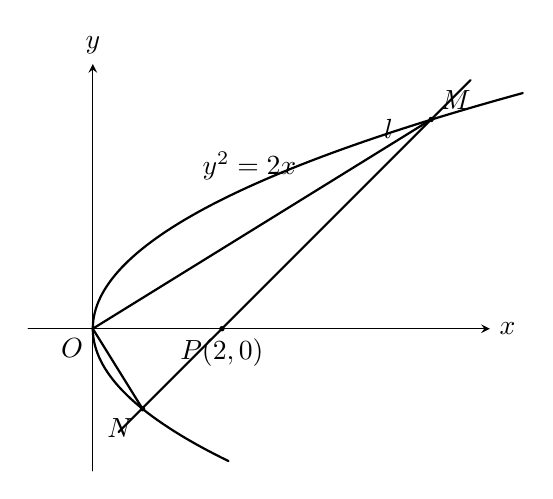
\begin{tikzpicture}[>=stealth, line cap=round, line join=round, scale=.82]
\draw[->] (-1.0,0)--(6.15,0) node[right] {$x$};
\draw[->] (0,-2.2)--(0,4.1) node[above] {$y$};
\node[below left] at (0,0) {$O$};
\draw[thick, domain=-2.05:3.65, samples=100, variable=\t]
  plot ({.5*\t*\t},{\t});
% A chord through the parabola's two marked points and the x-axis point P.
\coordinate (N) at (.77,-1.24); \coordinate (P) at (2,0); \coordinate (M) at (5.24,3.24);
\draw[thick] (.4,-1.6)--(5.85,3.85); % secant y=x-2 through P(2,0)
% Source also shows the two origin chords.
\draw[thick] (0,0)--(M) (0,0)--(N);
\fill (M) circle (1.2pt) (N) circle (1.2pt) (P) circle (1.2pt);
\node[above right] at (M) {$M$}; \node[below left] at (N) {$N$};
\node[below] at (P) {$P(2,0)$};
\node[above right] at (1.55,2.15) {$y^2=2x$};
\node[above left] at (4.8,2.8) {$l$};
\end{tikzpicture}
